\documentclass[a4paper,12pt]{article}
\usepackage[utf8]{inputenc}
\usepackage[T1]{fontenc}
\usepackage[italian]{babel}
\usepackage{graphicx}
\usepackage{hyperref}
\usepackage{amsmath}

\title{Relazione -- Settimana 1}
\author{Gruppo di Lavoro}
\date{\today}

\begin{document}

\maketitle

\section*{Introduzione e Obiettivi}
Durante la prima settimana di progetto, l'obiettivo principale è stato quello di organizzare in modo sistematico le informazioni necessarie, definire il piano di lavoro e iniziare l'approfondimento teorico. Abbiamo perciò istituito un ambiente di lavoro condiviso su \emph{Notion}, strutturato in diverse sezioni:
\begin{itemize}
    \item \textbf{Link e documentazione}: per raccogliere e categorizzare articoli, paper e video utili alla comprensione dei concetti chiave;
    \item \textbf{Domande e idee}: uno spazio dedicato al confronto su eventuali dubbi, spunti e proposte di miglioramento;
    \item \textbf{Pianificazione e scadenze}: una \emph{schedule} chiara, con date di consegna e priorità per ogni singola task, in modo da monitorare facilmente l’avanzamento del lavoro.
\end{itemize}

\section*{Ricerca e Studio Preliminare}
Per comprendere le basi teoriche del nostro progetto, abbiamo dedicato parte della settimana allo studio di:
\begin{enumerate}
    \item \textbf{Machine Learning e reti neurali}: analizzando il funzionamento di reti \emph{feed-forward}, reti ricorrenti e, in particolare, architetture di tipo \emph{Transformer}.
    \item \textbf{Word Embedding}: abbiamo revisionato i concetti di \emph{Word2Vec} e altri modelli associati, prendendo atto dei vantaggi e dei limiti di questi metodi rispetto ad approcci più recenti.
    \item \textbf{Sentiment Analysis}: approfondendo la letteratura e i casi di studio che utilizzano modelli moderni, tra cui \emph{BERT} di Google, come base per l'analisi del testo e la classificazione in positivo/negativo.
\end{enumerate}

Questa fase di ricerca è stata essenziale per capire i punti di forza di BERT rispetto a Word2Vec: in particolare, la capacità di cogliere i contesti linguistici in modo più ricco e la possibilità di \emph{fine-tuning} su dataset specifici.

\section*{Scelta di BERT e Struttura del Valutatore}
Una volta compresi i limiti dei metodi più classici, abbiamo optato per \emph{BERT} come modello principale per la \emph{Sentiment Analysis} e per la generazione di uno \emph{score} di affidabilità. A questo scopo, abbiamo realizzato lo schema di flusso del nostro \emph{valutatore}, illustrato in Figura~\ref{fig:flusso}.

\begin{figure}[h!]
    \centering
    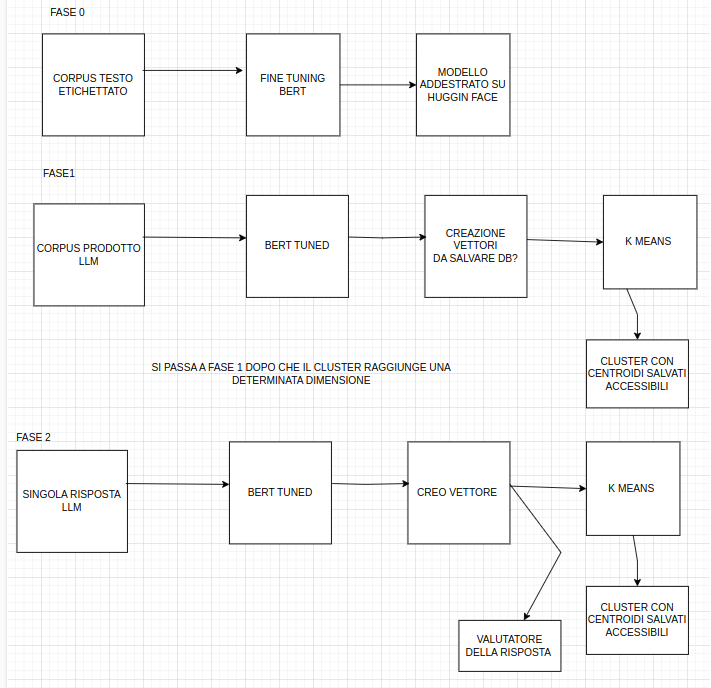
\includegraphics[width=0.8\textwidth]{image.png} % Sostituire con il nome effettivo del file immagine
    \caption{Schema del valutatore basato su BERT e clustering \emph{k-means}.}
    \label{fig:flusso}
\end{figure}

L’idea di fondo è la seguente:
\begin{enumerate}
    \item \textbf{Input dal LLM}: il testo prodotto da un \emph{Language Model} (LLM) viene passato a BERT, il quale fornisce in uscita:
        \begin{itemize}
            \item Un’etichetta di \emph{Sentiment} (positivo/negativo), che codificheremo come +1 o -1;
            \item Uno \emph{score} compreso tra 0 e 1, rappresentativo del livello di affidabilità della classificazione.
        \end{itemize}
    \item \textbf{Clustering con \emph{k-means}}: raccolte numerose risposte, utilizziamo l’algoritmo \emph{k-means} per creare due cluster principali (positivo e negativo), definiti dai loro centroidi. Ogni nuova risposta, una volta classificata e vettorizzata, sarà assegnata a uno dei due cluster in base alla distanza dal rispettivo centroide.
\end{enumerate}

\section*{Fine-Tuning e Dataset}
Abbiamo compreso che, per ottenere risultati efficaci, \emph{BERT} andrà \emph{raffinato} (\emph{fine-tuning}) su un dataset \emph{ad hoc}. Poiché vogliamo applicare il modello a un caso d'uso specifico (ovvero la valutazione di risposte generate da LLM), sarà necessario:
\begin{itemize}
    \item Creare un dataset di frasi o risposte etichettate manualmente (positivo/negativo) e arricchite di eventuali metadati utili.
    \item Addestrare BERT su questi dati, in modo che apprenda le peculiarità del linguaggio e dei contesti specifici del nostro dominio.
\end{itemize}
La costruzione del dataset avverrà nelle prossime settimane, durante le quali definiremo le linee guida di etichettatura per garantire coerenza e uniformità.

\section*{Prossimi Passi}
Al termine di questa prima settimana, abbiamo discusso l’idea con il professor Ferretti, che ha approvato la direzione presa. Ci ha inoltre suggerito di effettuare i primi test su \emph{Google Colab} utilizzando la versione base di BERT, per poi passare ai \emph{cluster} del dipartimento, dotati di maggiori risorse computazionali. 

Resta ancora aperta la questione relativa alla \textbf{dinamicità dei cluster}: non è chiaro se, in fase di utilizzo a regime, ogni nuova risposta debba aggiornare il modello di clustering oppure se il clustering debba essere “statico” dopo una prima fase di addestramento. Questo aspetto sarà oggetto di approfondimento nelle prossime iterazioni, quando potremo misurare l’impatto di un aggiornamento dinamico sulla precisione e sulla stabilità del sistema.

\section*{Conclusioni}
In sintesi, la prima settimana di lavoro ci ha permesso di:
\begin{itemize}
    \item Organizzare la collaborazione e la gestione dei materiali tramite \emph{Notion};
    \item Studiare i concetti chiave di \emph{Machine Learning}, \emph{reti neurali} e \emph{Transformer};
    \item Identificare \emph{BERT} come modello di riferimento per la \emph{Sentiment Analysis} e per l’estrazione di uno \emph{score} di affidabilità;
    \item Definire la struttura complessiva del valutatore, basato sul \emph{fine-tuning} di BERT e sul clustering \emph{k-means}.
\end{itemize}

Nei prossimi giorni, procederemo alla creazione del dataset di addestramento e ai primi test su \emph{Google Colab}, in modo da validare le nostre ipotesi progettuali e valutare l’efficacia di \emph{BERT} nel contesto specifico del nostro sistema di valutazione.

\end{document}
